\chapter{Graphics}
To create the graphics we need to first analyse Viner's work to see the
characteristics that need to be replicated; we then should create a method for
drawing the grid of polygons. The vertices of the polygons need a method to be
offset and the number of vertices in the polygon changed.

Where Viner's work was a static image and our is dynamic; we should also
consider how the image changes as parameters change. The points must move
smoothly between configurations to give the illusion of being in that
`landscape' rather than that of a series of static images.

\begin{figure}[H]
    \centering
    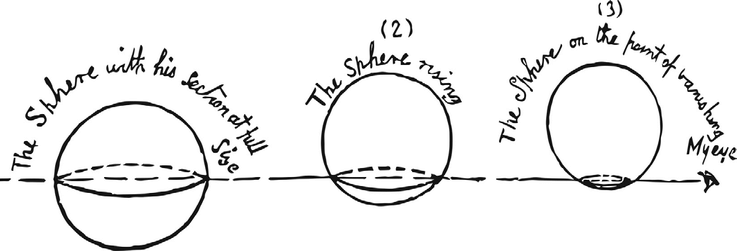
\includegraphics[width=0.5\textwidth]{flatlandsphere}
    \caption{Figure reproduced from Flatland \citep[p.112]{abbott1885flatland}}
\end{figure}

The landscape is not just 2D, parameters each constitute a dimension, when one
is changing we see a 2D slice of the multi-dimensional world as in the book
`Flatland' ``You cannot indeed see more than one of my sections, or Circles, at
a time; for you have no power to raise your eye out of the plane of Flatland;
but you can at least see that, as I rise in Space, so my sections become
smaller. See now, I will rise; and the effect upon your eye will be that my
Circle will become smaller and smaller till it dwindles to a point and finally
vanishes.'' \citep[p.112]{abbott1885flatland} A shape (polygon in this instance,
sphere in the book) cuts through the plane to show `slices' of itself. Here we
are in `flatland' and the parameter space we create allows us to see the work as
slices of a higher-dimensional shape (than 2D). 

\begin{figure}[H]
    \centering
    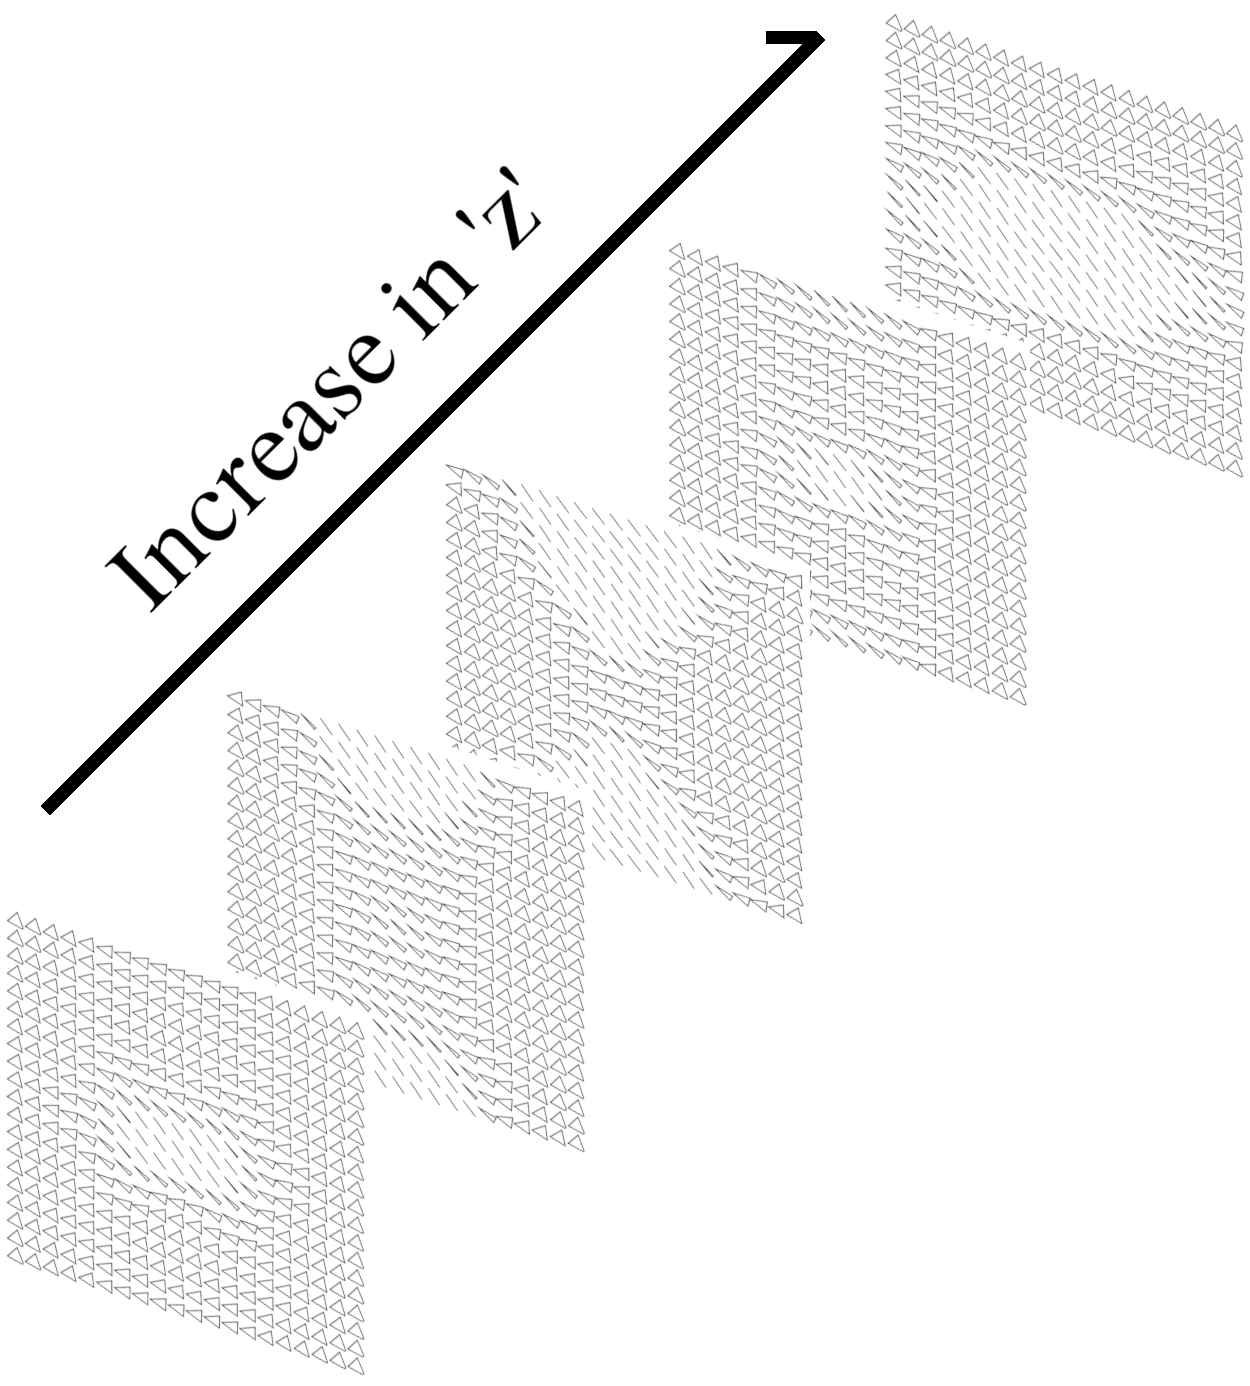
\includegraphics[width=.5\textwidth]{3d}
    \caption{Here the `z' parameter increases, each `layer' is morphed between
    smoothly}
\end{figure}

\section{Anatomy of the Work}
Viner's pen plotter work was created by a set of programs, created in
\verb|FORTRAN| using a set of subroutines called \verb|PICASO| (PIcture Computer
Algorithms SubroutineOriented) \citep{lycett_2016}, this was essentially a
graphics library, similar to what we are using processing / p5js for. This
library was presented as part of J. A. Vince as part of their PhD.
\verb|PICASO|'s use by Viner isn't well documented but the manual has
subroutines for transforming vertices according to some rules (affine
transformations, morphs between shapes) \citep{picaso_manual}. Some pencil notes
on Viner's work indicate there was mathematical thinking going on in
the development, but without access to the code listings, it is hard to say
exactly how the images were generated.

\section{Polygons}
\label{Polygons}
One aspect the program should be able to do is to grow and shrink polygons
between different numbers of vertices. Viner's work uses different numbers of
vertices between images, so we should be able to reproduce this by allowing a
smooth transition between polygons. 

\begin{figure}[H]
    \centering
    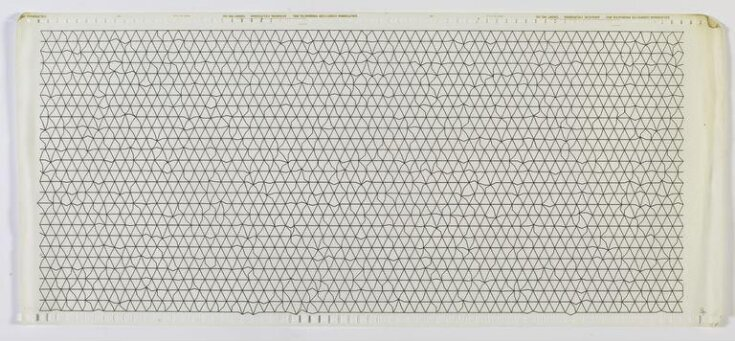
\includegraphics[width=0.45\textwidth]{triangleViner}
    \hspace{0.2cm}
    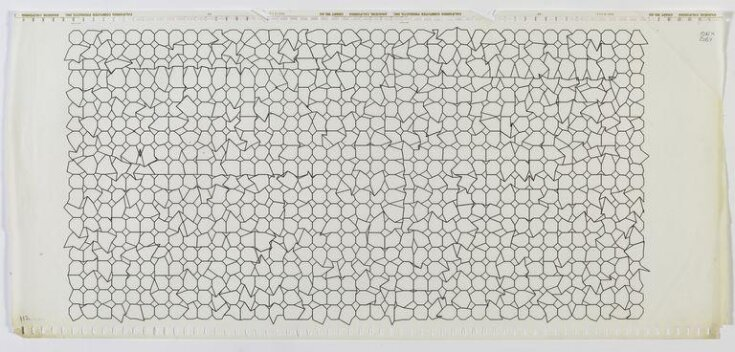
\includegraphics[width=0.45\textwidth]{octagonViner}
    \caption{Two Viner pieces showing the use of polygons}
\end{figure}


To achieve this a polygon is inscribed on a circle. The points of this polygon
of $n$ vertices on the circle are simply given by $$(x, y) = (\cos(\frac{2k
\pi}{n}), \sin(\frac{2k\pi}{n})) \text{ where } k = 0, 1, \ldots, \lfloor n
\rfloor$$ 

We can note that for integer values of $n$ the rotation will be complete, for
non-integer values of $n$ this also works given that we used the floor of $n$ as
the limit giving us an incomplete polygon, we can use the fact we have the first
coordinate to close the shape. This gives us the smooth transition between
integer values of $n$.

\begin{figure}[H]
    \centering
    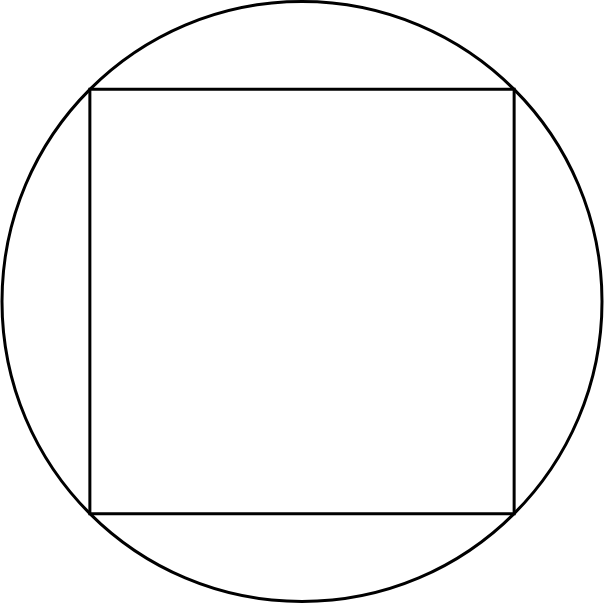
\includegraphics[width=0.2\textwidth]{n4}
    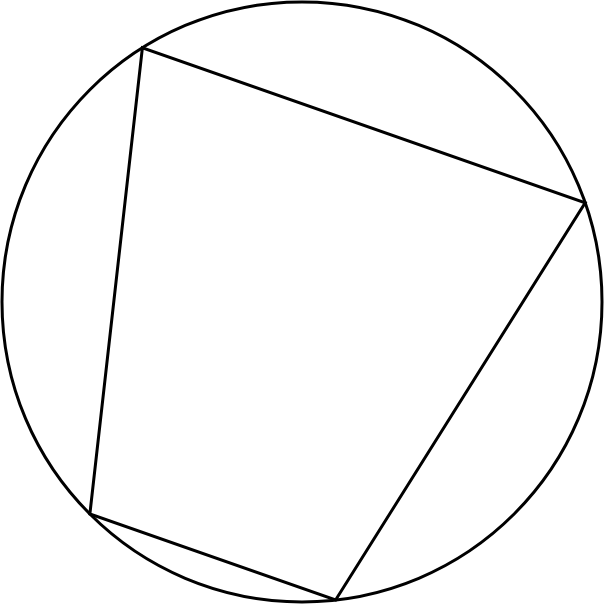
\includegraphics[width=0.2\textwidth]{n35}
    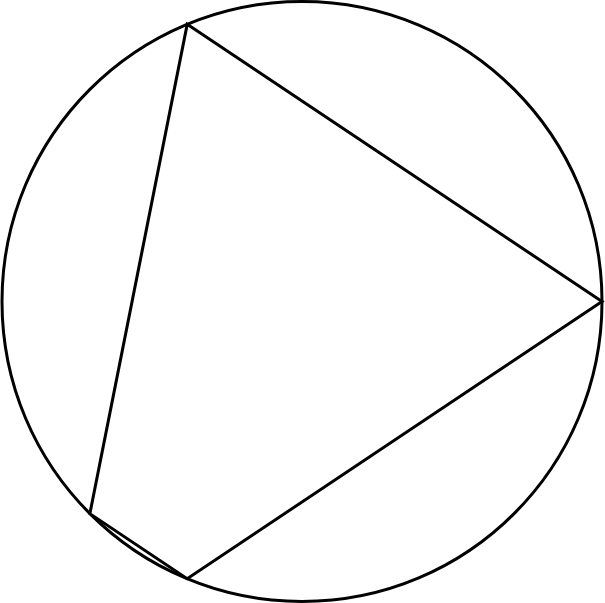
\includegraphics[width=0.2\textwidth]{n32}
    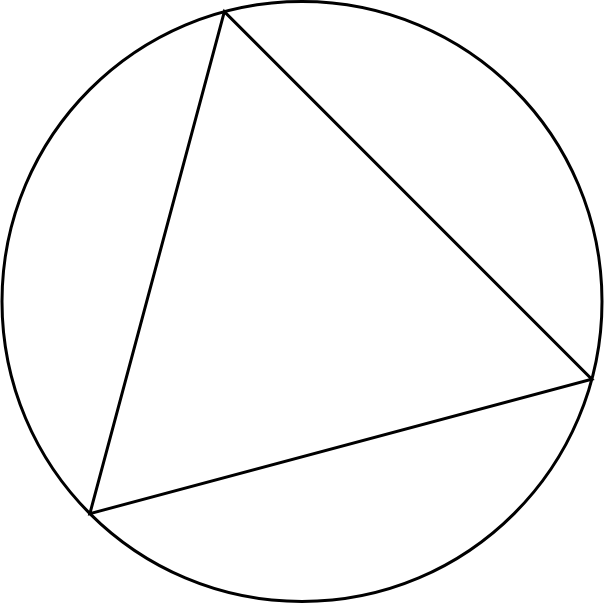
\includegraphics[width=0.2\textwidth]{n3}
    \caption{Starting at $n=4$ the shape deforms through $n=3.5$, $n=3.2$ and
    finally $n=3$}
\end{figure}

In code we can implement this as such:
\begin{lstlisting}[language=JavaScript]
// center
let x = innerWidth/2;
let y = innerHeight/2;
let n = 4;
let r = 300;

let theta = (3*QUARTER_PI) - TWO_PI/n;
dTheta = TWO_PI/n;

beginShape()
    for (i = 0; i <= n; i++) {
        theta += dTheta;
        vertex(x + r*cos(theta), y + r*sin(theta));
    }
endShape(CLOSE);
\end{lstlisting}

An offset to each $(x,y)$ pair can be made inside the loop. A function to limit
the maximum offset should be created too. Here is an example of using noise to
calculate the offsets.

\begin{center}
\begin{tabular}{c}
\begin{lstlisting}[language=JavaScript]
ox = limit(noise(sx*cos(theta), sz)*10, 2*gridSize);
oy = limit(noise(sy*sin(theta), sz)*10, 2*gridSize);
\end{lstlisting}
\end{tabular}
\end{center}

The limit function is a simple sine calculation ensuring the offsets don't become
larger than $\pm$ 2 times the grid size.

\begin{lstlisting}[language=JavaScript]
function limit(value, amplitude) {
    return amplitude * sin((PI / amplitude) * value);
}
\end{lstlisting}

\section{The Grid}
The motif of a grid with changes present across the image is central to Viner's
work, so a method of drawing this should be created.

The centre point of the grid is assigned a coordinate \verb|x,y,z| which is what
is modified by the user when interacting with the program. The polygons around
this point are calculated from that offset using the following calculation:

\begin{center}
\begin{tabular}{c}
\begin{lstlisting}[language=JavaScript]
sx = (x + ((gridSize+gridSpacing) * ((cols/2) - i)));
sy = (y + ((gridSize+gridSpacing) * ((rows/2) - j)));
sz = (z + (gridSize * (cols/2)));
\end{lstlisting}
\end{tabular}
\end{center}

Where \verb|i,j| is the column and row value of the point, \verb|cols, rows|
are the total number of columns, rows, and \verb|gridSize| is the pixel size
of the grid and the similarly for the \verb|gridSpacing|. 

This leads to the idea of a `view window' of which the parameters in the program
describe only the central polygon and the parameters for the others in the grid
are calculated.

The grid should also be centred on \verb|x,y| so calling a translate before
drawing any points should be done:
\begin{center}
\begin{tabular}{c}
\begin{lstlisting}[language=JavaScript]
translate((innerWidth/2) - x, (innerHeight/2) - y);
\end{lstlisting}
\end{tabular}
\end{center}

Here a grid is prepared with fixed parameters that distort around
\verb|x=0, y=0|. This point is fixed, and when the program is interacted with
the world moves beneath the player rather than the point of distortion being
changed, the grid displayed is reflecting the `terrain' visible from the centre
point.

\begin{figure}[H]
\centering
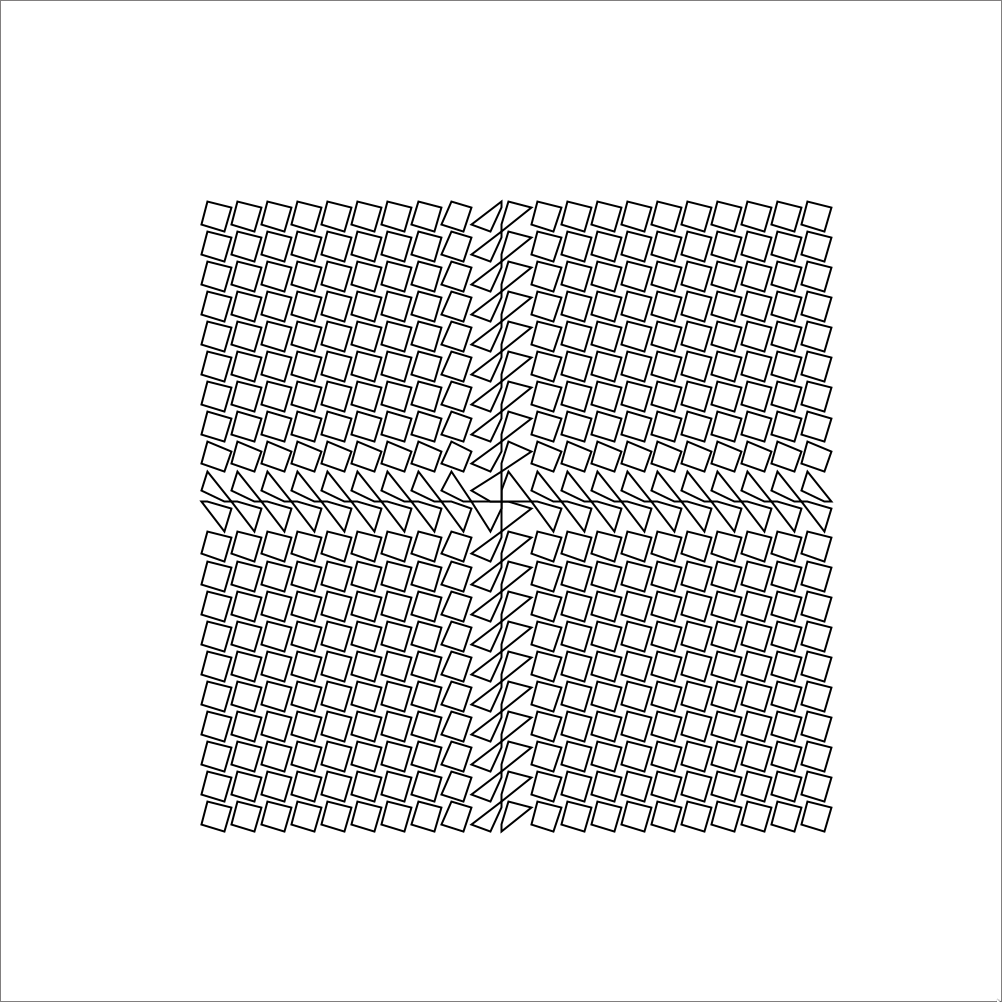
\includegraphics[width=.4\textwidth]{PoC3}
\hspace*{0.5cm}
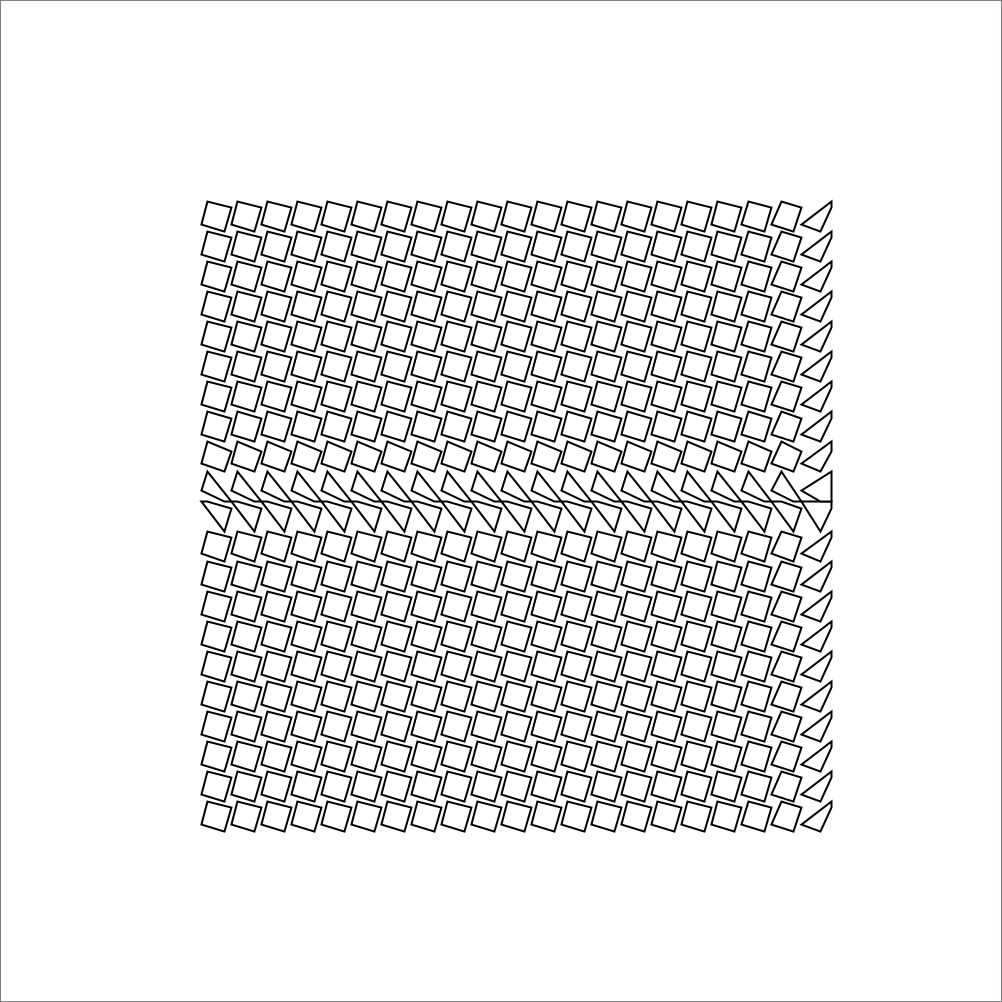
\includegraphics[width=.4\textwidth]{PoC2}
\caption{The user presses `a' for a short time, decreasing the `x' parameter}
\label{demomovement}
\end{figure}

We then use \verb|sx, sy| to draw a polygon using the method described
previously, with the \verb|sx, sy| as the centre.

Another possibility was considered to make the grid a simple series of vertices
and have a method to draw lines between them according to some rule. This was
ultimately rejected due to much more complexity when moving between a number of
vertices in the polygon dynamically.

\section{Landscape Generation}
\label{landgen}
% Talk about landscape analogy
The program should generate a `landscape' or `topography', this is an analogy for
a space that has a continuous change of the parameters across them. `Landscape'
is apt because we're exploring a set of features generated by the program much
like if you were to look at a topographic map. The user should have the feeling
of moving through space like this, more than simply increasing some parameter
and immediately seeing a change throughout the grid.

% Talk about explorations into proc gen, dynamical systems etc.
This is the main question of how the program will work on a technical level, how
can we create an algorithm or mathematical model that explores the spaces that
Viner's work set out to create?

We need to be able to take the parameters of the program and reduce them down to
a single value for use to create an offset or number of vertices in a shape.

Dynamical systems may be of interest and allow for a system to be created where
a state evolves into other states following some rules. These states can be
deterministic which is important for the objective that we have of recall, but
can also be chaotic, which may be aesthetically desirable. Similarly, fractals
may be useful for their self-similarity. Given we're working with a grid, the
ability to have self-similar properties may be aesthetically useful. Neither of
these however would be particularly flexible as one function would need to be
picked and used throughout the whole program. Also, to model a landscape with
the right-sized `regions' may prove difficult.

This leads to the choice between having each session using the software be
either random in some sense or the same every time. Ideally given a random
option to fulfil the ability to recall previous sessions, a seed would be given.

For this reason, noise is a good solution, the majority of noise implementations
allow you to specify a seed and thus have this property of reproducibility
between sessions. Graphical implementations of noise are often created with the
express reason of looking natural and organic.

\subsection{Noise}
A desirable property is that of a smooth gradient between extremes, or
defined regions in which values are high and low. This will help to demarcate
`regions' on a map (think, the mountains, the foothills, and the plains). 

\verb|p5js|'s built-in noise function is a Perlin noise generator. You can pass
it up to three coordinates. Perlin noise was designed for computer graphics
\footnote{And won an Oscar for "allow[ing] computer graphics artists to better
represent the complexity of natural phenomena" \citep{nyu_perlin}}, and is
fairly simple, generating a random grid of vectors and then computing the dot
product vectors and their offsets, then finally interpolating to create a more
smooth image \citep{10.1145/566570.566636}.

\verb|p5js| also provides a \verb|noiseDetail()| method that provides some
control over the 'texture' of the noise. Also for reproducibility
\verb|noiseSeed()| allows the programmer to set a seed value for the noise.
The \verb|noise()| function takes three coordinate arguments and outputs a
number between $0-1$

\begin{figure}[H]
\centering
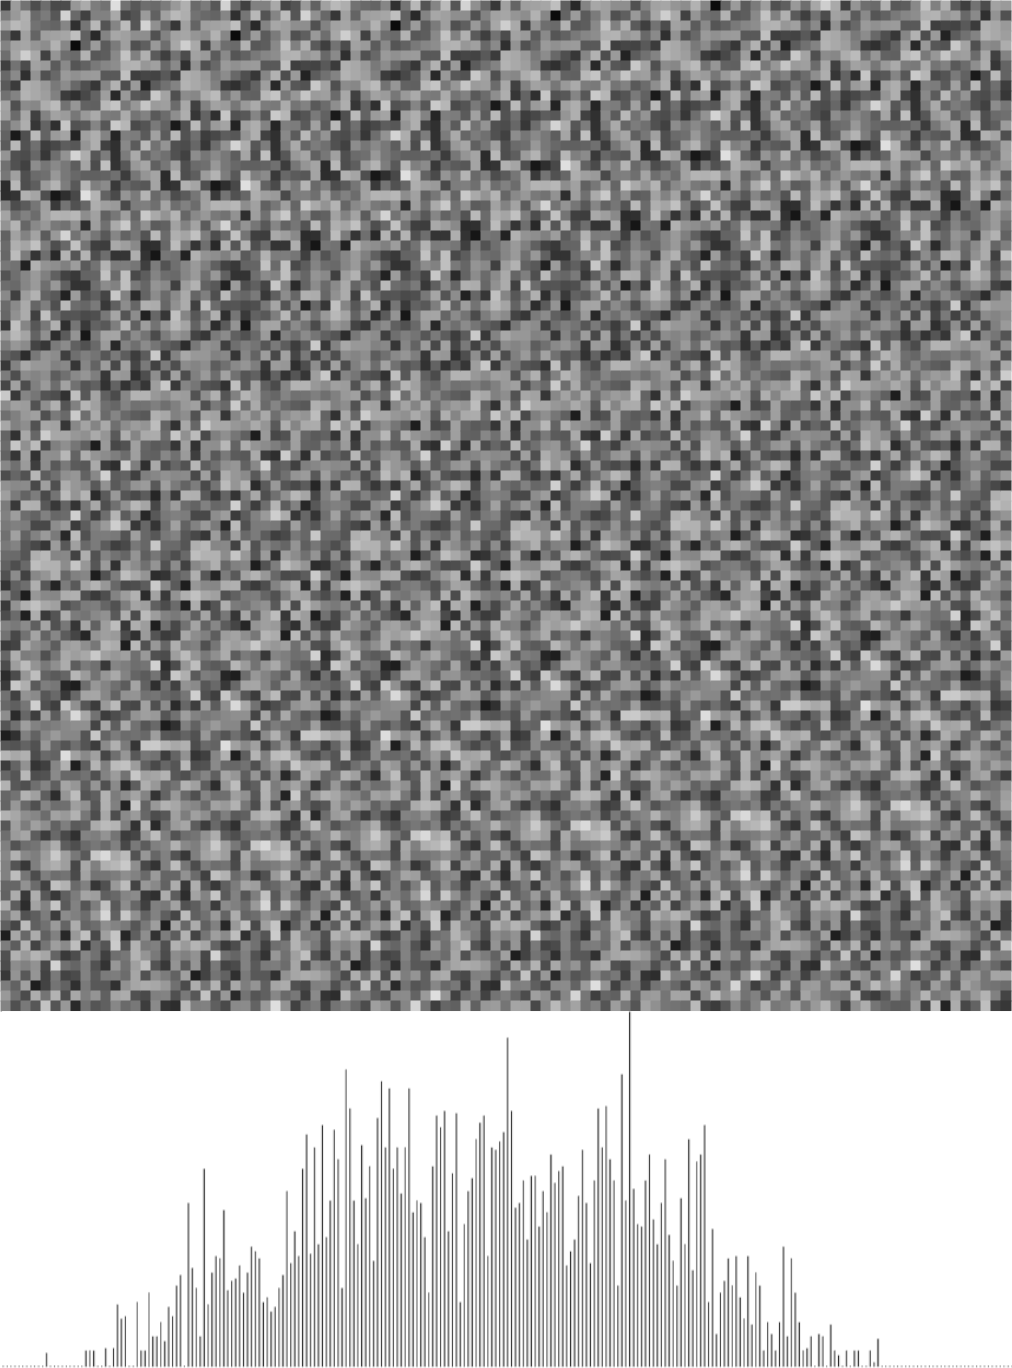
\includegraphics[width=.4\textwidth]{noiseDefault}
\hspace{0.2cm}
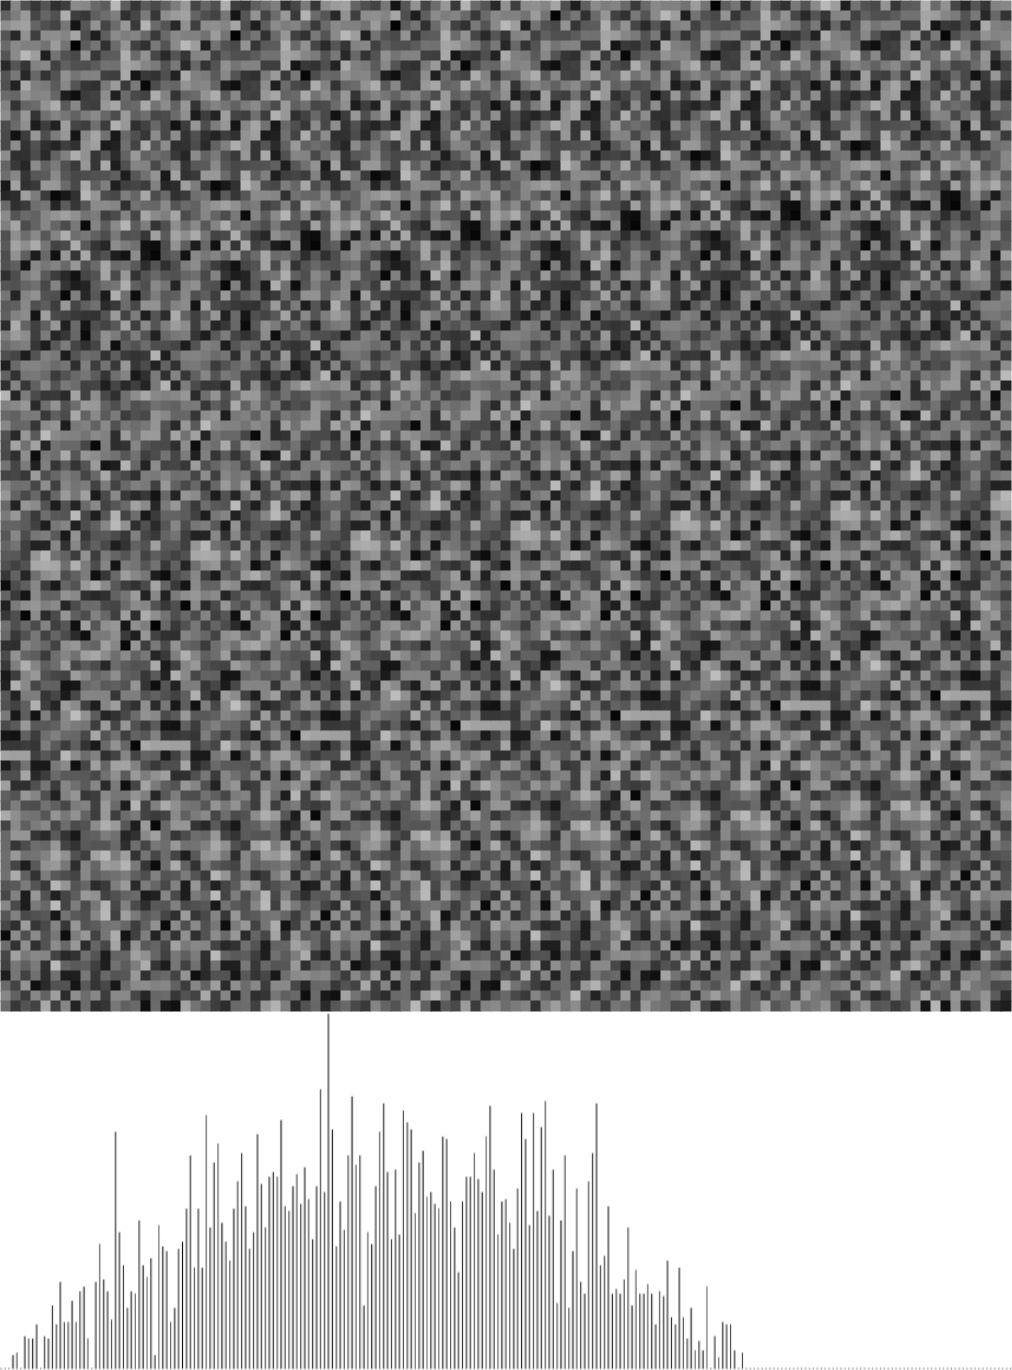
\includegraphics[width=.4\textwidth]{noiseDetail2halfFalloff}
\caption{Two Perlin noise samples (one default the other with
noiseDetail(2, 0.5) with the same seed, histograms plotted beneath show
that the adjustment makes the image overall darker}
\end{figure}

One option we may wish to be able to have is `quantising' the noise to some set
of values. For example, we may wish to have areas of a certain value of $n$ for a
polygon. This can be achieved by mapping the noise from $0-1$ to $0-n$ and
rounding to the closest integer. This was happening implicitly with the
histogram above. We can see that because the distribution is uni-modal the most
common values will be those towards the centre of the range.

\begin{figure}[H]
\centering
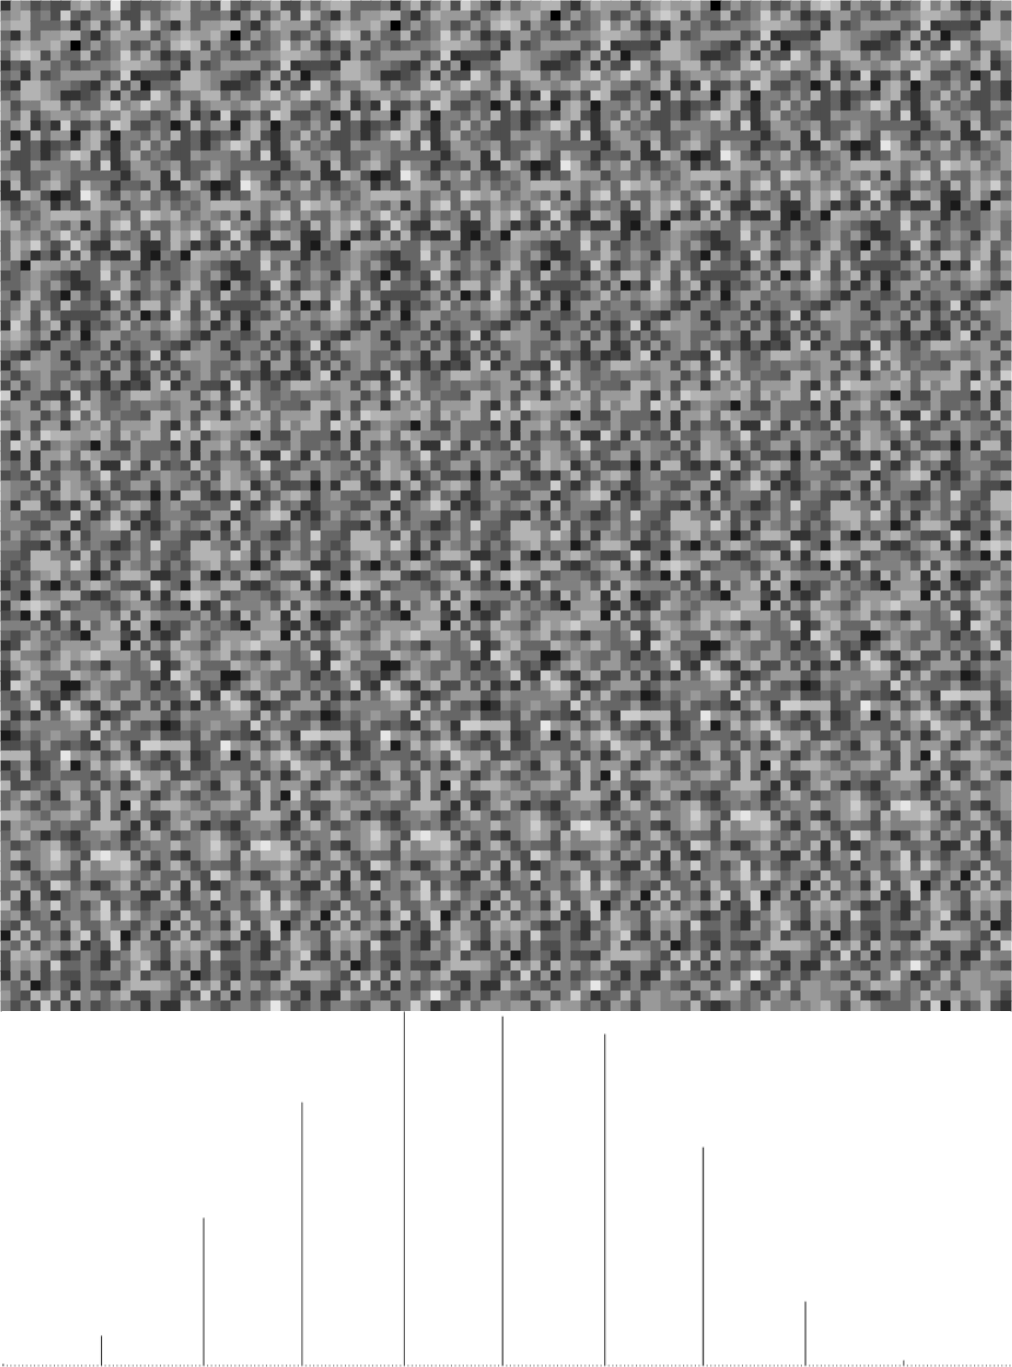
\includegraphics[width=.4\textwidth]{noiseQuantised}
\caption{This sample contains only ten colours}
\end{figure}

\begin{figure}[H]
\centering

\includegraphics[width=.4\textwidth]{noiseScaleUnquantised}
\hspace{0.2cm}

\includegraphics[width=.4\textwidth]{noiseScaleQuantised}
\caption{Unquantised and quantised noise at 0.001 noiseScale}
\label{0.001scale}
\end{figure}

This effect is much more obvious when the noise scale is a lot smaller, this
would then allow for discrete regions between two integer values for a
parameter. What if we don't want discrete regions and instead something more
like a multi-modal distribution i.e. smoothing applied between edges?

We can use a waveform such as the sawtooth to achieve `smoothing' by using it to
estimate rounding, adding the value to the wave produces something approximating
the `staircase' function of piece-wise rounding. To do this we can use additive
synthesis:

$$x + \frac{1}{\pi} (-\sum^\infty_{k=1} \frac{\sin(2k \pi x)}{k})$$

To use this in code we take only some number of terms, this determines the
accuracy of the rounding, the lower the more `smooth', i.e. inexact the output:
\begin{lstlisting}[language=JavaScript]
function approx_round(value, terms) {
    let result = value;
    
    var innerSum = -sin(2 * PI * value);
    for (i = 2; i <= terms; i++)
        innerSum += (sin((i * 2) * PI * value) / i)

    result += innerSum / PI;

    return result;
}
\end{lstlisting}

\begin{figure}[H]
\centering
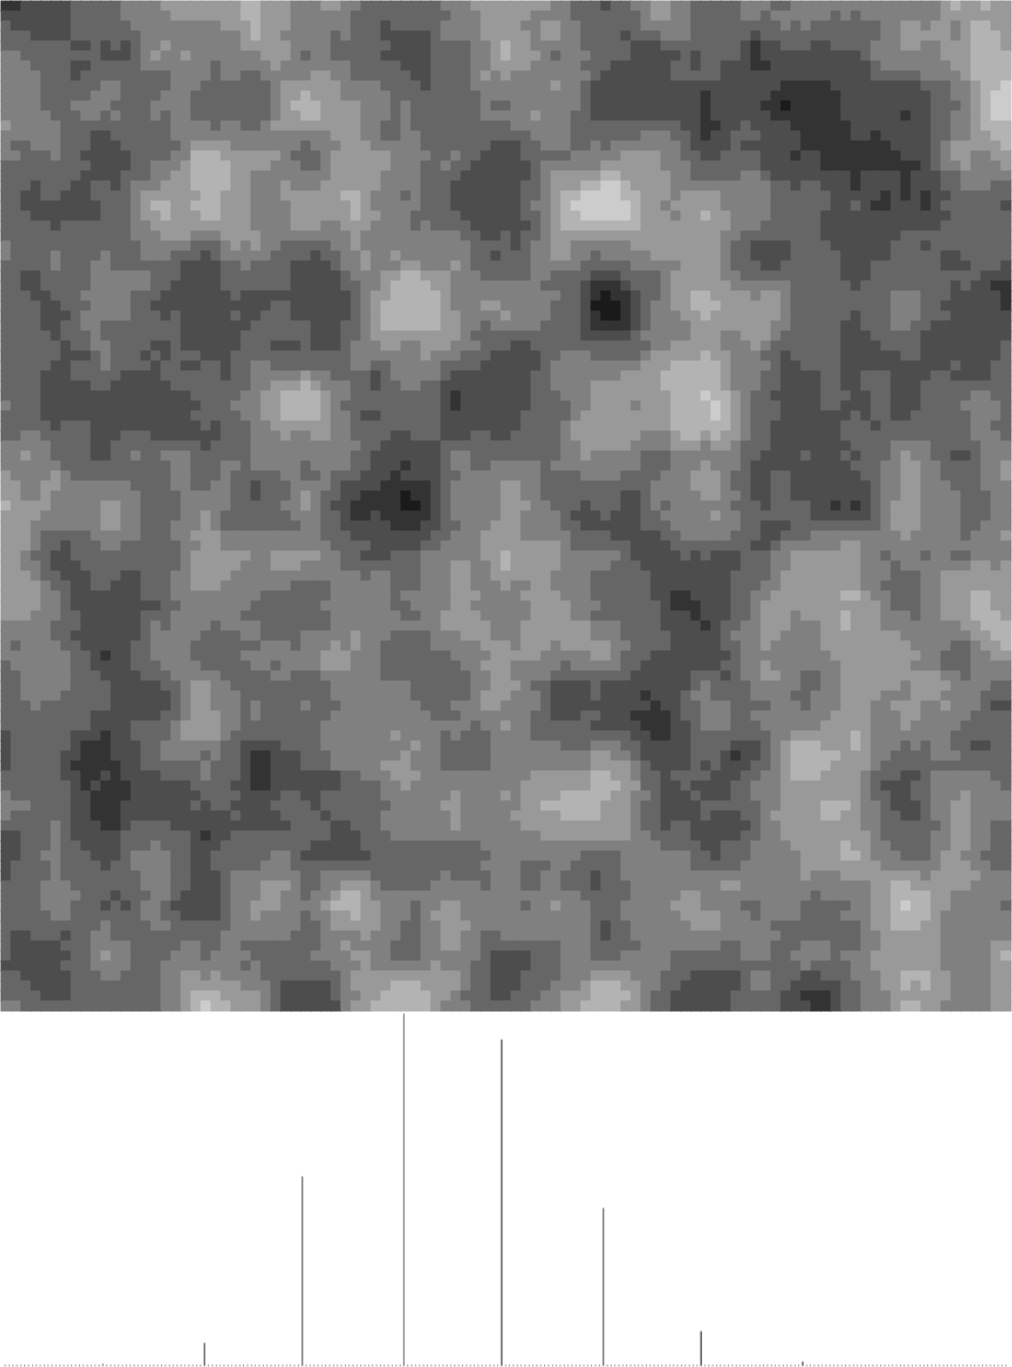
\includegraphics[width=.2\textwidth]{noiseRounded}
\hspace{0.2cm}
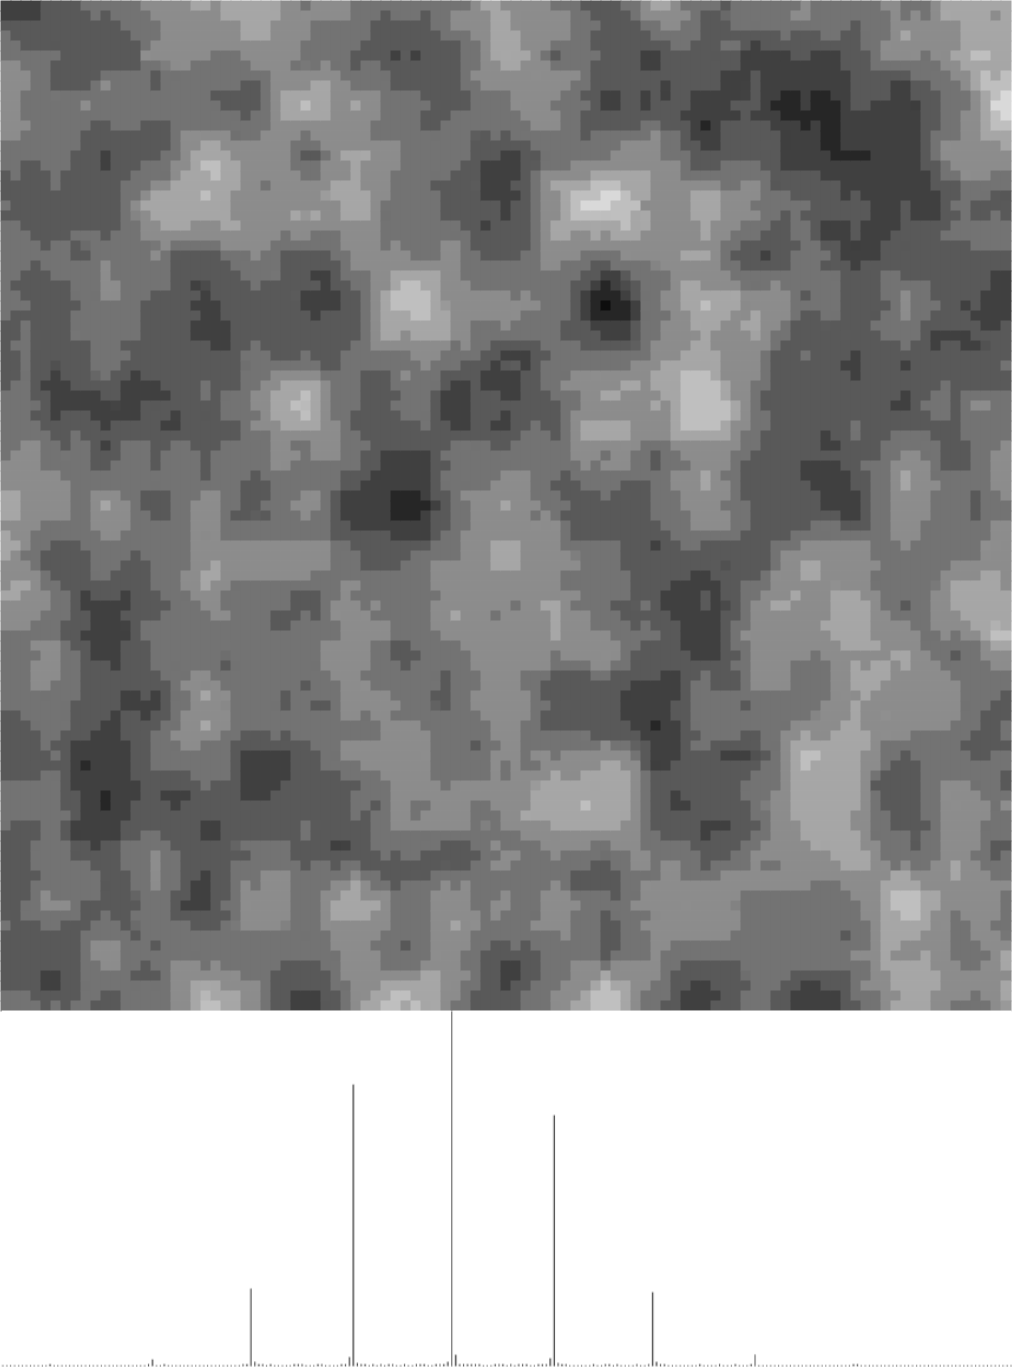
\includegraphics[width=.2\textwidth]{noiseAlmostRounded100}
\hspace{0.2cm}
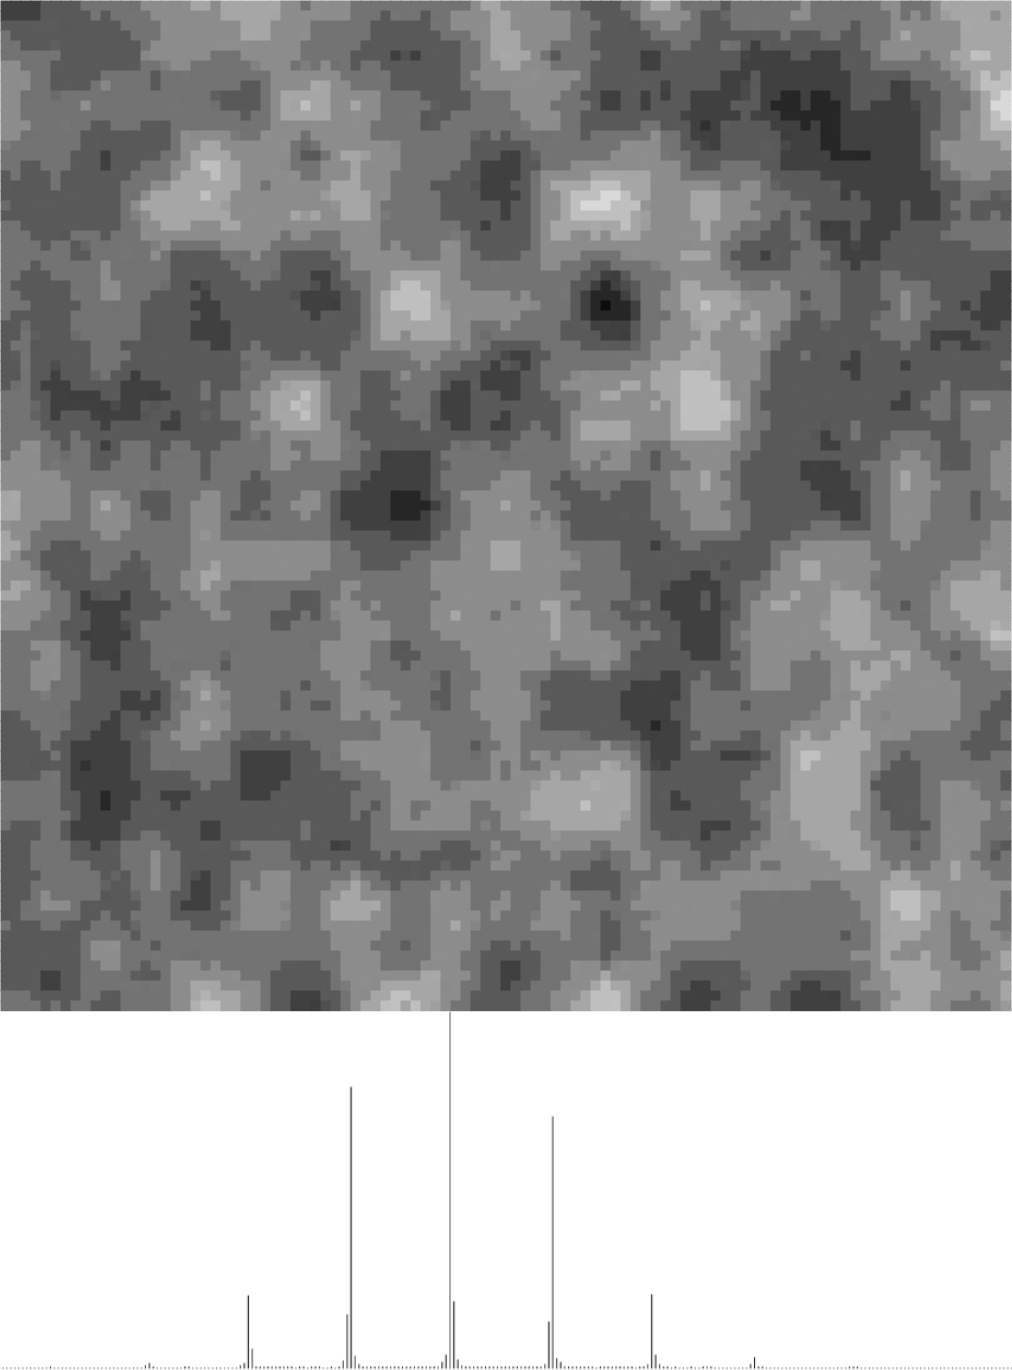
\includegraphics[width=.2\textwidth]{noiseAlmostRounded20}
\hspace{0.2cm}
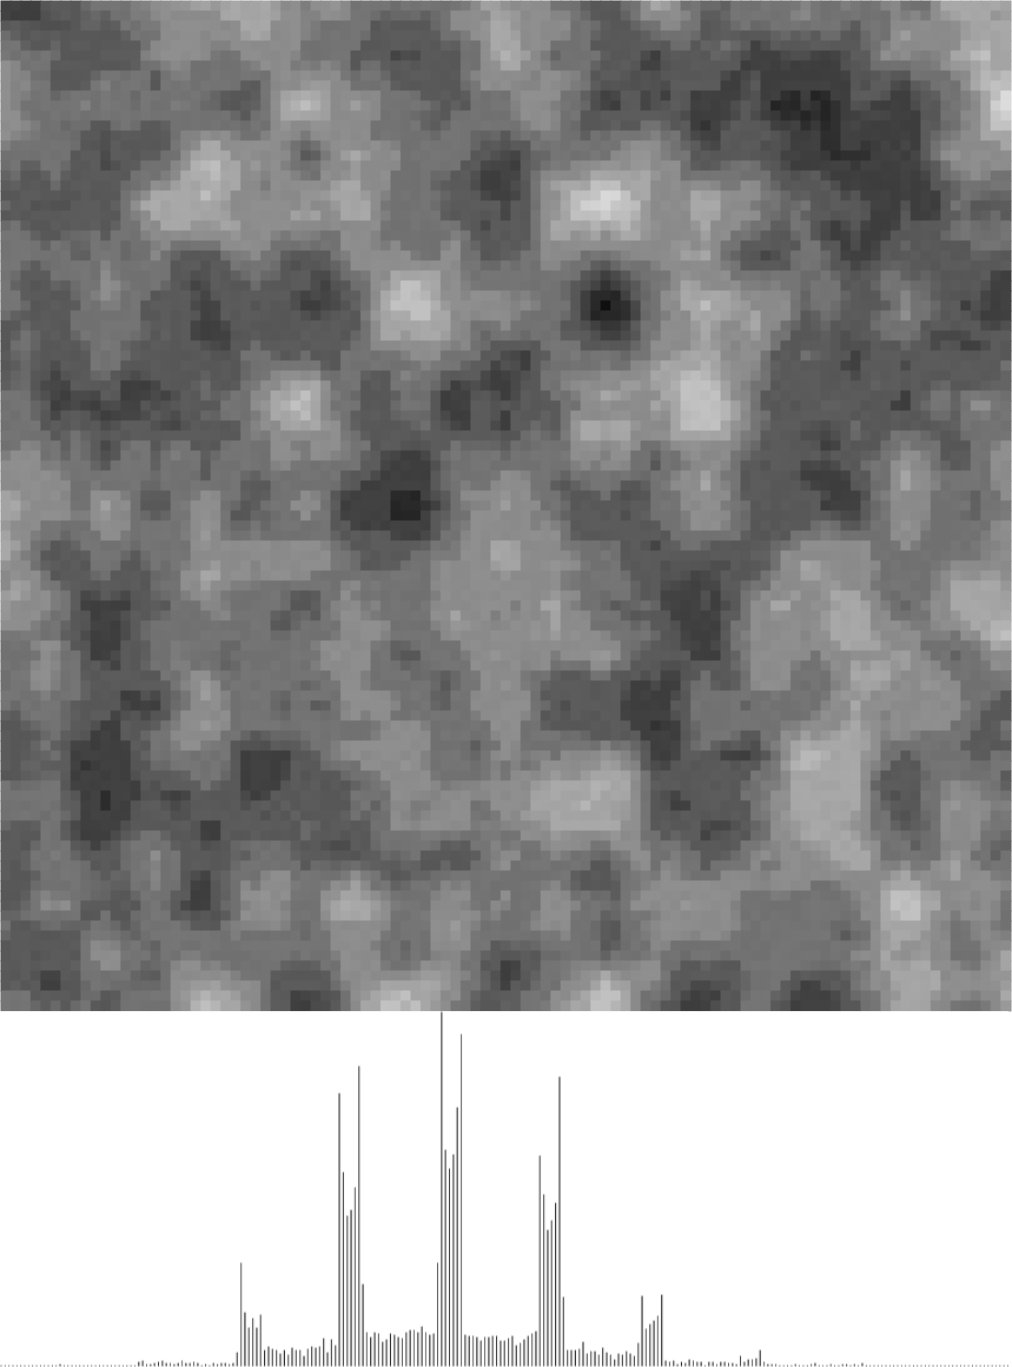
\includegraphics[width=.2\textwidth]{noiseAlmostRounded1}
\caption{Rounded discretely, Terms = 100, Terms = 20, Terms = 1}
\end{figure}

At such a large scale the difference is hard to perceive but when using the
example in \autoref{0.001scale} there's a clear `smoothing' in the boundaries.

\begin{figure}[H]
\centering
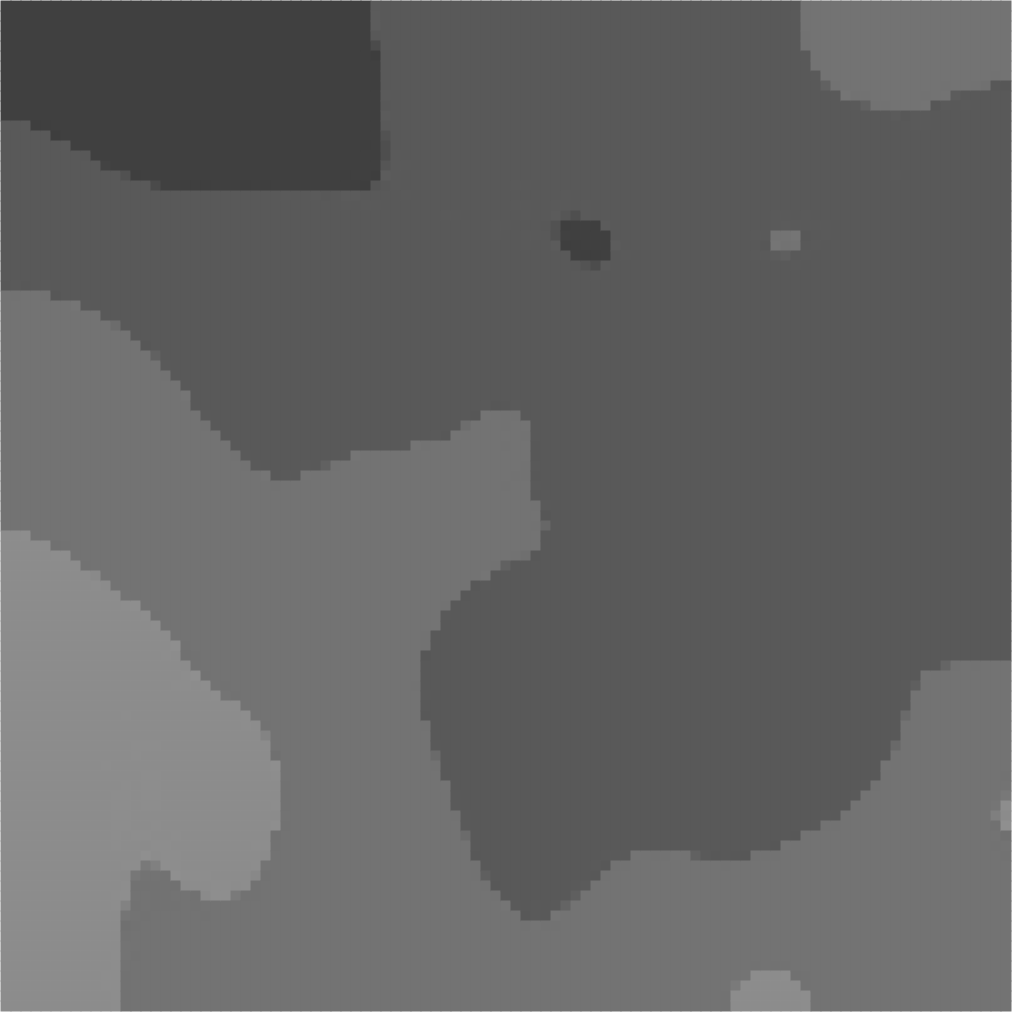
\includegraphics[width=.3\textwidth]{noiseScaleAlmost}
\hspace{0.2cm}

\includegraphics[width=.3\textwidth]{noiseScaleAlmost10}
\hspace{0.2cm}
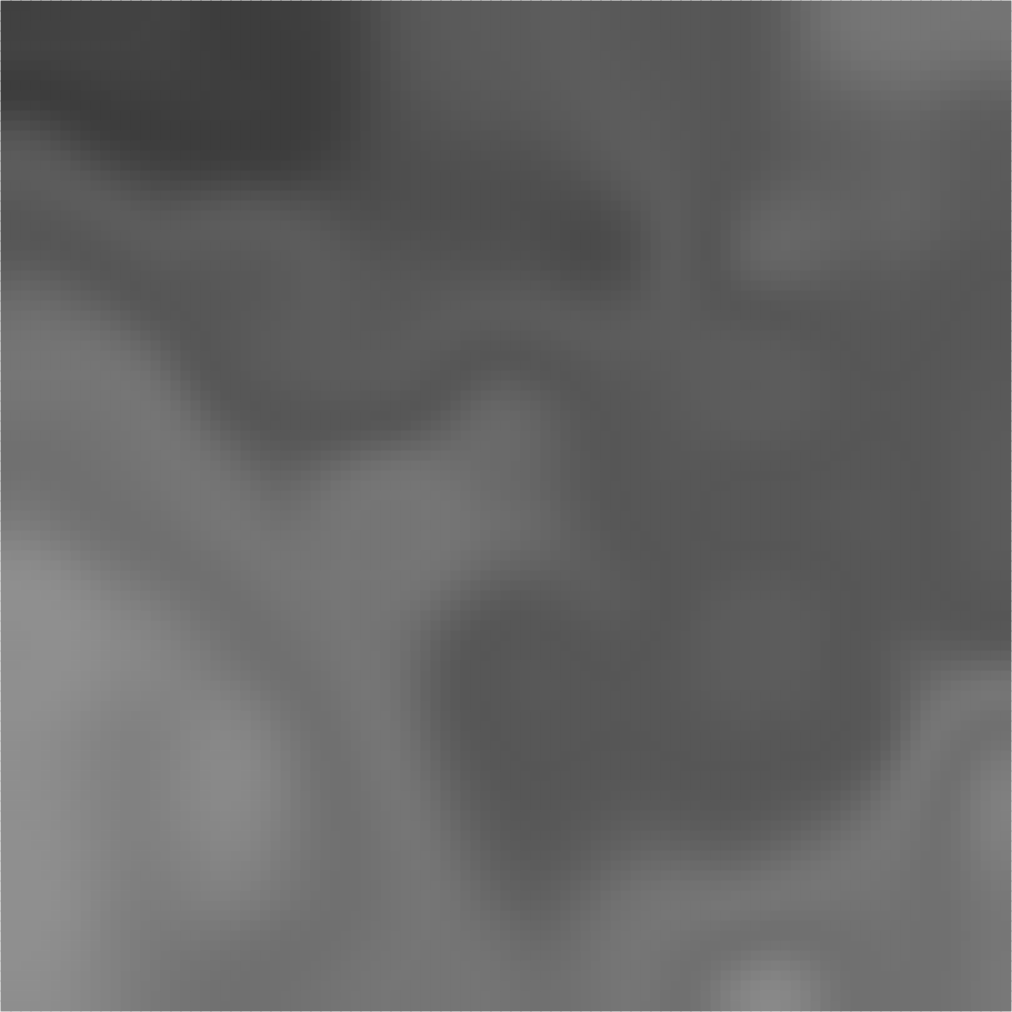
\includegraphics[width=.3\textwidth]{noiseScaleAlmost1}
\caption{Terms = 100, Terms = 10, Terms = 1}
\end{figure}

Implementing this such that noise controls the number $n$ (vertices in a
polygon) we can get results like this (note that the background is shaded darker
for lower values of $n$ and lighter for higher values of $n$)
\begin{figure}[H]
\centering
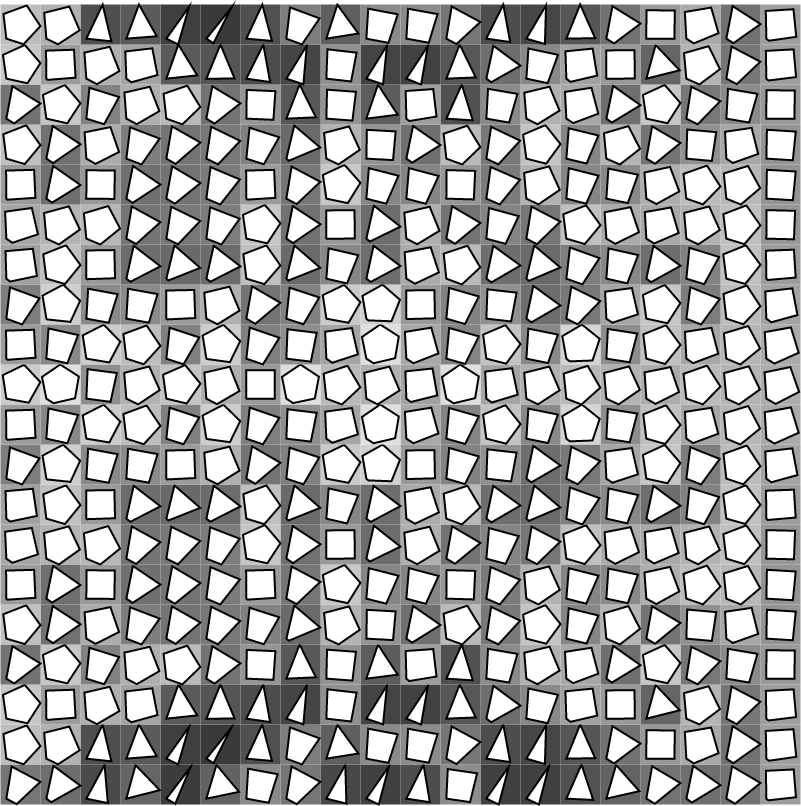
\includegraphics[width=.4\textwidth]{noisewithPolygons}
\hspace{0.2cm}
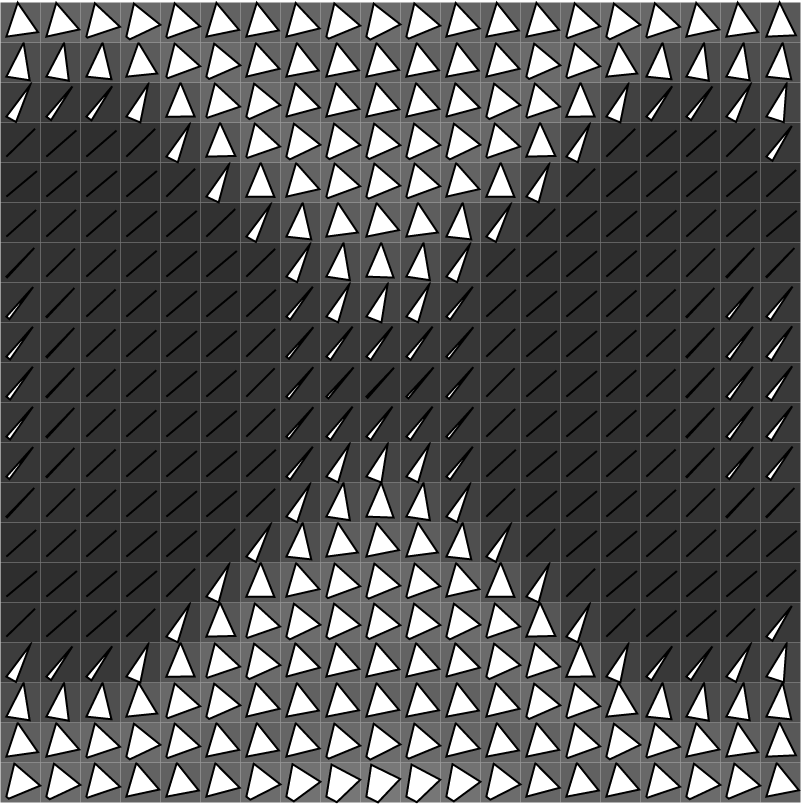
\includegraphics[width=.4\textwidth]{noisewithPolygons1term}
\caption{Terms = 20, Terms = 1}
\end{figure}

With user interaction, this scheme creates the feeling of moving through regions
of these different values of $n$ and the parameter for the number of terms
allows for adjustments to be made about how `hard' or `soft' the borders between
these regions look.

This approach is, I believe somewhat novel, as most techniques for adjusting
noise is usually done at a whole-image level. This method is point-wise and thus
can work for each polygon or vertex in the grid we have defined. In the field of
signal processing the concept of `quantisation noise' is similar but reversed,
taking a continuous signal and analysing the error in the digital discrete
signal. Here we are designing a function for an artistic application, and I do
not think that it has application to the field of signal processing as it works
on discrete to discrete transformations and not continuous to discrete.

\section{Integration}
%TODO tie together the whole thing
These parts then tie together to make the whole graphical system, the polygons
are drawn at each point in the grid and given an offset by the noise; this is
all drawn within a \verb|push()| and \verb|pop()| so as to not affect the
history tree (detailed later). Here is one iteration of the loop through the
columns and the rows:

\begin{lstlisting}[language=JavaScript]
// calculate x y and z values for the current polygon
sx = (x + ((gridSize+gridSpacing) * ((cols/2) - i)));
sy = (y + ((gridSize+gridSpacing) * ((rows/2) - j)));
sz = (z + (gridSize * (cols/2)));

// From section on polygons and noise, generate a number from 1 to 6 for
// the number of verticies
n = approx_round(map(noise(sx*0.001, sy*0.001, sz*0.001), 0, 1, 1, 6), 1);

let theta = (3*QUARTER_PI) - TWO_PI/n;
dTheta = TWO_PI/n;

beginShape()
    for (k = 0; k <= n; k++) {
        theta += dTheta;
        // Calculate offsets to points
        ox = limit(noise(sx*cos(theta)*0.001, 
                         sz*0.001)*noiseMultiplier, 
                   2*gridSize);

        oy = limit(noise(sy*sin(theta)*0.001, 
                         sz*0.001)*noiseMultiplier, 
                   2*gridSize);

        // Points on the circle
        xc = sx + ox + gridSize * cos(theta);
        yc = sy + oy + gridSize * sin(theta);
        
        // draw the vertex
        vertex(xc, yc);
    }
endShape(CLOSE);
\end{lstlisting}

In this code snippet we can see that most of the above code is replicated but
with some changes in multipliers (e.g. values in noise are multiplied by 0.001)
these are changes made to produce aesthetic results in the final output.

\section{Navigation}
Because this program deals with a set of parameters that change over time, it is
a good idea to look at concepts for navigating higher-dimensional space that
already exist; in this, we can learn how other people have approached this. If we
imagine each parameter in the program as a spatial dimension, there is a body of
knowledge available regarding this because many fields rely on large
multivariate data; for example the field of machine learning for example deals
with very high dimensional data in feature vectors.

Tools like `\verb|ggobi|' exist to help explore multi-variate data
\citep{swayne:dsc2003} which tend to disregard spacial relations of points in
favour of clustering based on shared properties. A novel method is that of the
grand tour, through which a series of scatter plots are projected orthogonally
into 2D subspaces from the higher-dimensional space and moved then between
continuously to describe multi-variate data \citep{asimov1985grand}.

Whilst these approaches are useful for data, what we're dealing with here is
generating spaces to explore, these spaces are less about trends in data and
more about geometric exploration through many continuous parameters. In this, we
want all of the data of the parameters to be visible at once, meaning these data
visualisation methods are not as useful for our purposes.

\begin{figure}[H]
    \centering
    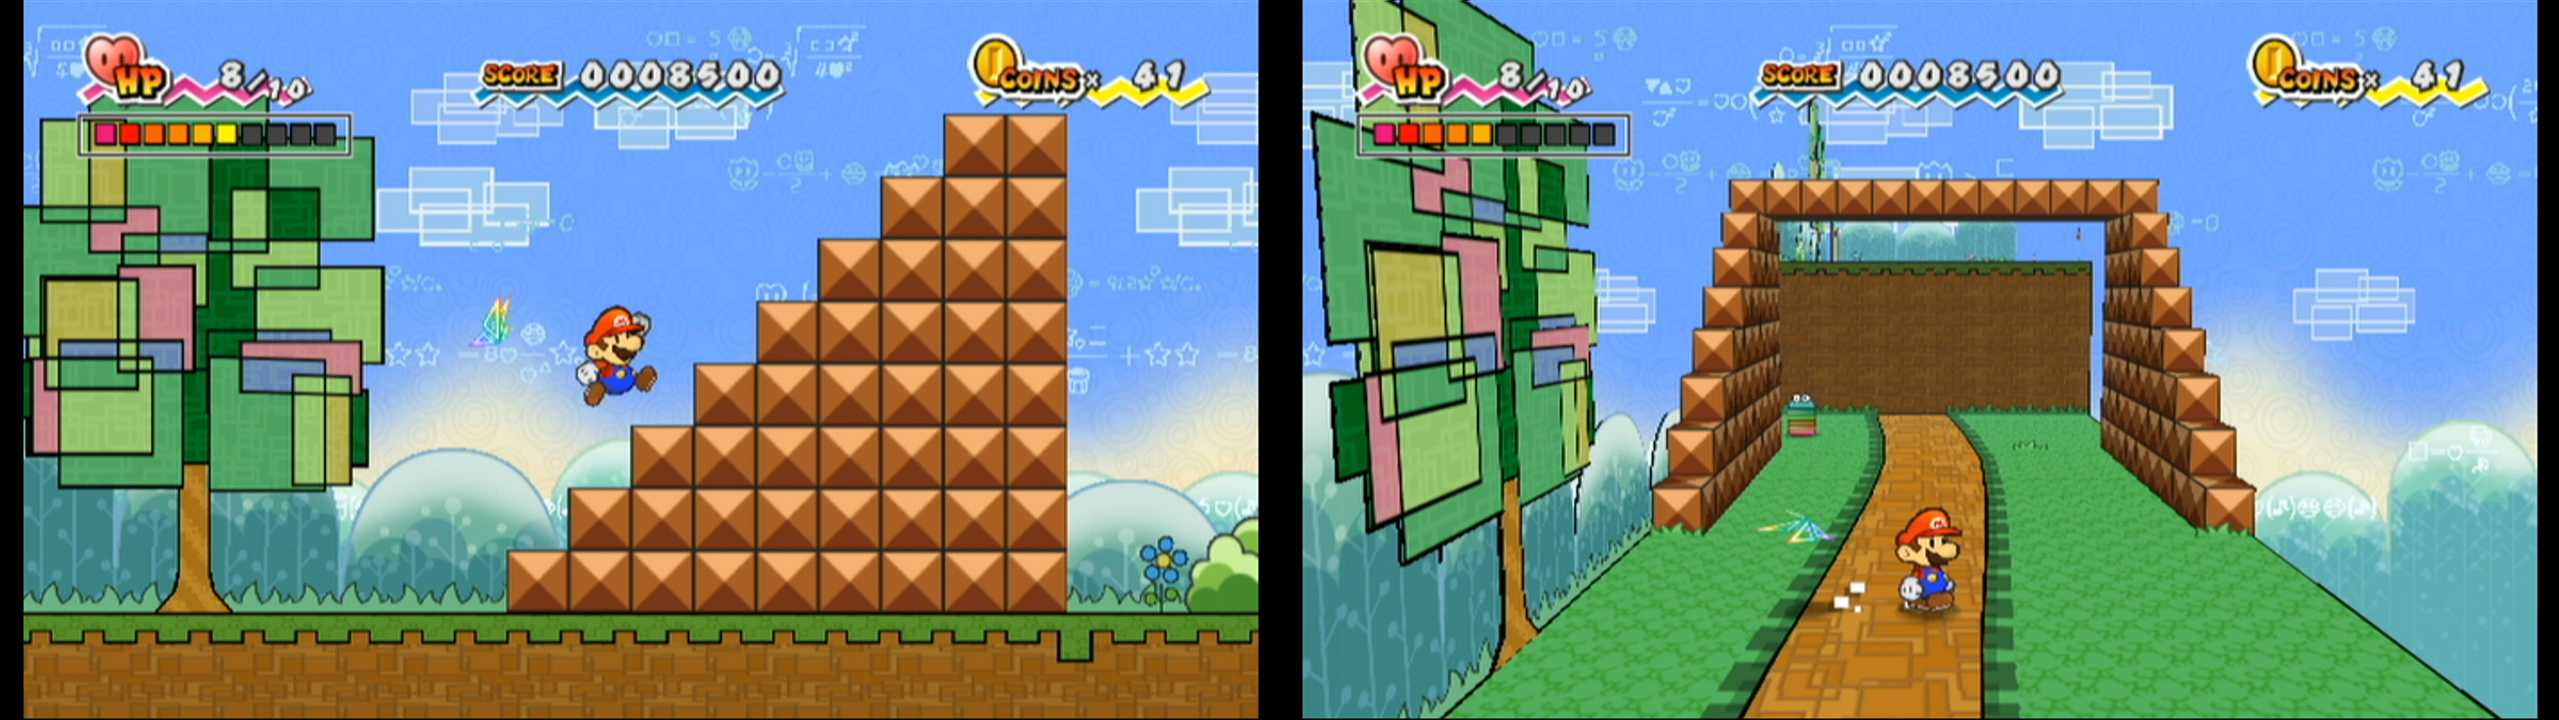
\includegraphics[width=0.9\textwidth]{marioturns}
    \caption{Mario turns $90^\circ$ around the z-axis (\emph{Super Paper Mario
    (2007) pub. Nintendo})}
\end{figure}

Video games also have explored higher-dimensional spaces. An interesting concept
is that of 2D characters being able to navigate 3D spaces.  \emph{Super Paper
Mario (2007)} for the Nintendo Wii is an example of this, the player can turn
the world 90 degrees about the y-axis to explore the depth of the z-axis and
progress through the game. An extension of this from a 3D character turning 90
degrees and being able to explore the 4th Dimension is present in the unreleased
game \emph{Miegakure} in which the player can move through the 4th Dimension
using the controller, to help orient the player a graphic\footnote{Which the
developer tells me is based on an astrolabe} is displayed below the controlled
character showing the position of the slice of the 4D world, these slices are
like the 2D slices we can see in MRI imaging but in 3D.

Whilst these worlds explore pre-made or procedurally generated assets (models,
textures, sprites, etc.), and this program instead will explore moving through
various parameters, ideas for how the user can interface with the program to
understand where exactly they are.

\subsection{Graphical Prompts}
A simple idea to allow the user to recall where in the parameter space they were
could be a spider / radar plot or parallel coordinates plot. For our intents, these
are the same as we're only displaying a single set of parameters the spider plot
is just a `round' version of the parallel coordinates plot. This could exist on
the screen somewhere and change as the user moved around the parameter space,
and would allow the user to recall approximately where they were. The spider
diagram could also be `extruded' from how it looked at every point to create a
3D model that represented how you moved through the parameters.

However, this method might be unintuitive and remove the user from the main
focus of the program. The grid should reflect the changes in the parameters in a
way that becomes apparent with some exploration; making this somewhat redundant.
Other options like this can be considered for other projects, but here there is
no need. The idea of history existing in a third axis is interesting for further
applications, however. 

\subsection{Controls}
The above-mentioned video games allow for the user to move through space by
only letting the user worry about at most 3 dimensions at any one time and
regarding the others as static when moving through them, this allows the user to
control the movement with traditional controls (either a games controller or
keyboard and mouse).

In \autoref{demomovement}, the \verb|WASD| style of control, popular in video
games is used. This will be familiar to people who have played video games but
not to people who haven't, for whom it may make sense to use the arrow keys.
It's also important to note that in that particular demo the `d' key increases
\verb|x|, this gives the feeling that the world is moving `beneath' you instead
of you moving the world itself; if the controls were flipped such that `d'
decreased \verb|x|, it would instead feel like you were moving the world. This
is extended for other buttons. For example, the use of `e' and `c' are common to
move up and down in video games (e.g. Second Life). A similar pattern using
`ijkl' is present on the right-hand side of the keyboard that allows both hands
to be used.

In the end to control all of the parameters the keys `w, a, s, d, e, c, q, z, i,
k' were used. Each controlling a different parameter. `w, a' corresponding to y,
`s, d' corresponding to x, `e, c' corresponding to z, `q, z' to the spacing of
the grid, and 'i, k' to the amount of noise displacement given to each point.

Another option would be something like an array of knobs, these could encode one
parameter each, and as a scientific instrument be `tuned'. However, this relies
on specialist hardware. This would probably feel less like `moving' through
space and more exploring a range of possibilities.

\section{User Interface}
The final graphical element to consider is how the user interacts with the HTML
elements that control various functions. I created: an upload and download button
for interaction with the history; a mute button and volume slider for the audio;
and a help screen that explains the key controls and what the program is.

\begin{figure}[H]
    \centering
    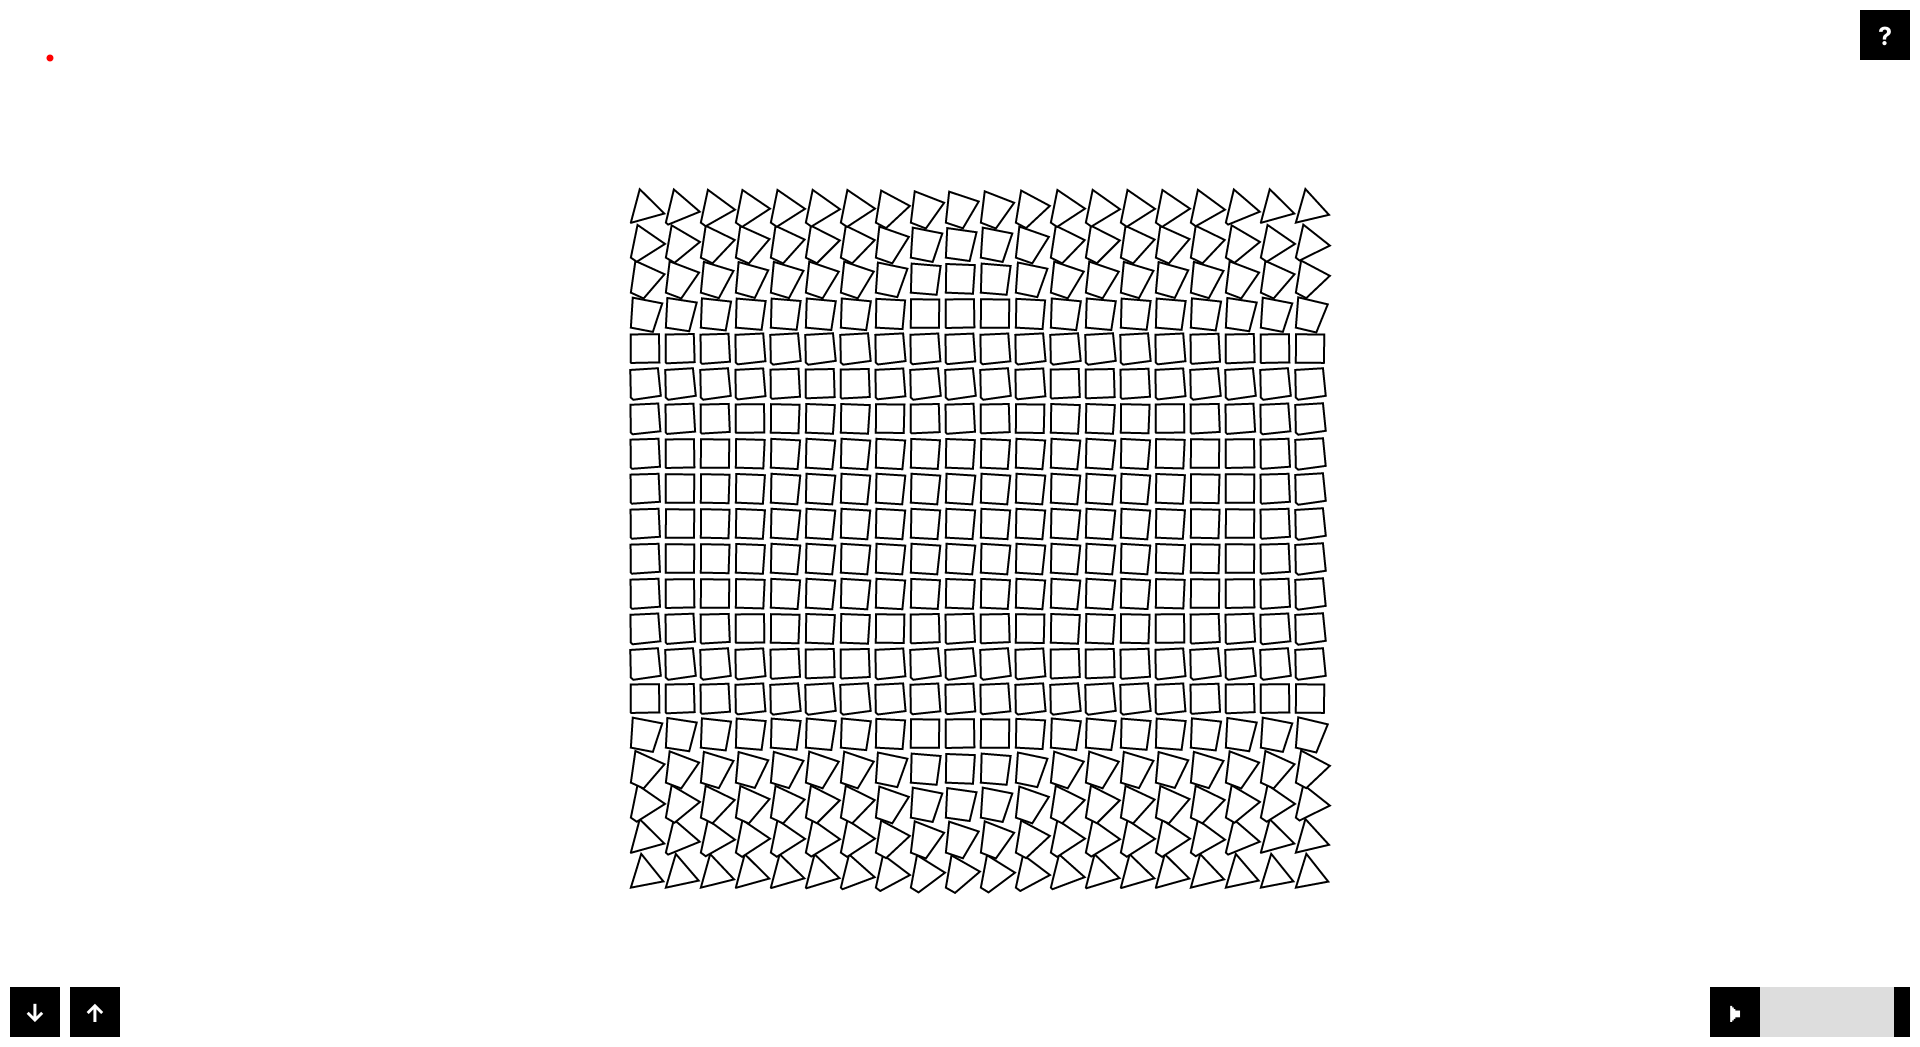
\includegraphics[width=1\textwidth]{webinterface}
    \caption{Web interface with buttons}
\end{figure}

I decided to keep the buttons simple, and without text to not distract
from the main graphical part of the program. They also animate when the user
hovers over them (they gain a black border and grey background) to indicate they
are can be clicked.

\begin{figure}[H]
    \centering
    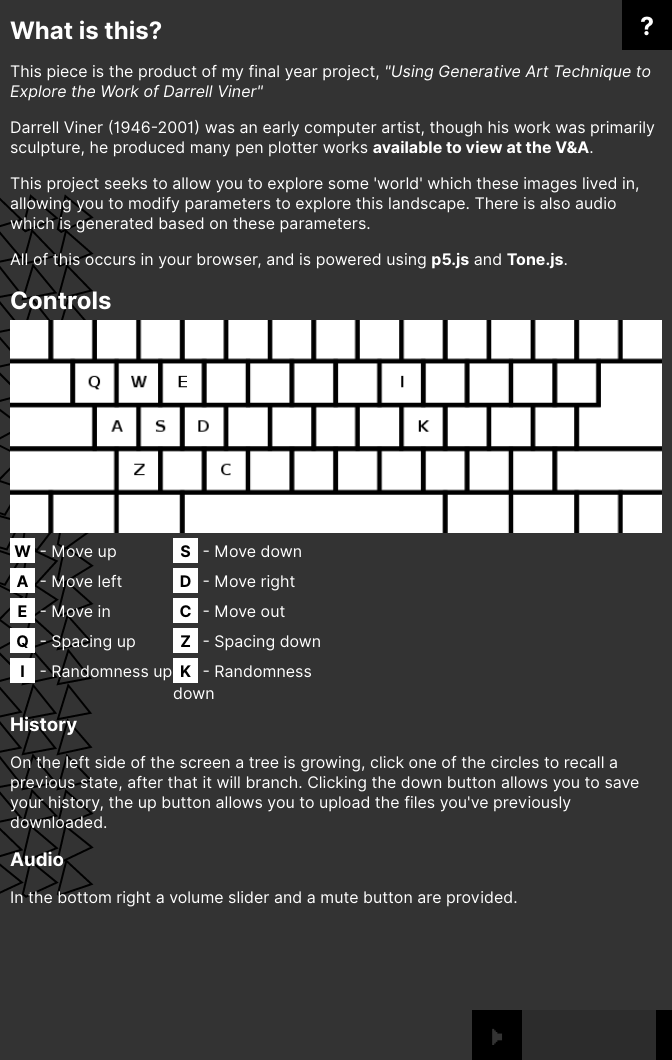
\includegraphics[width=0.5\textwidth]{helpmenu}
    \caption{Help menu}
\end{figure}

The help menu expands when the `?' button in the top right is hovered and
retracts when the user un-hovers the help menu. The background is slightly
transparent to not block the rest of the program. I produced a graphic of
a keyboard to help explain where the keys are located on the users' computer and
a flex-box list of keys (that adapt to different screen widths). I also included
a short explanation of how the history tree works and what the audio controls
do.
